\begin{problem}{가장 큰 정사각형}{표준 입력(stdin)}{표준 출력(stdout)}{2\,초}{512\,MB}

건덕이는 $N \times N$ 크기의 격자판을 가지고 있다. 격자판의 각 칸은 $1 \times 1$ 크기이며, 검정 또는 흰색으로 칠해져 있다.

격자판의 가장 왼쪽 위는 $(1, 1)$이고, 가장 오른쪽 아래는 $(N, N)$이다.

건덕이는 아래와 같은 규칙에 따라 격자판을 움직여 재배열할 수 있다.

\begin{itemize}
  \item 맨 오른쪽 열을 떼어내 격자판의 가장 왼쪽에 붙인다.
  \item 맨 아래 행을 떼어내 격자판의 가장 위쪽에 붙인다.
  \item 행, 열을 떼어내 붙일 때, 격자판이 $N \times N$ 크기를 유지하게끔 붙여야 한다.
\end{itemize}

건덕이는 임의의 횟수만큼 격자판을 재배열해 가장 큰 검은색 정사각형을 만들려고 한다. 건덕이를 도와 답을 구해주자.

\InputFile
첫 번째 줄에 $N$이 주어진다. $(1 \leq N \leq 12)$

두 번째 줄부터, $N$줄에 걸쳐서 격자판의 상태가 주어진다. 각 칸은 공백으로 구분되어 있으며, 1은 격자판이 검정색으로 칠해져 있는 경우, 0은 흰색으로 칠해져 있는 경우이다.

\OutputFile
격자판을 적절히 재배열해 만들 수 있는 가장 큰 검정색 정사각형의 넓이를 출력한다.

\Examples

\begin{example}
\exmp{
3
1 0 1
0 1 0
1 0 1
}{%
4
}%
\exmp{
3
1 1 0
0 0 0
1 1 1
}{%
4
}%
\end{example}

\Note
\begin{center}
\begin{tabular}{lllll}
  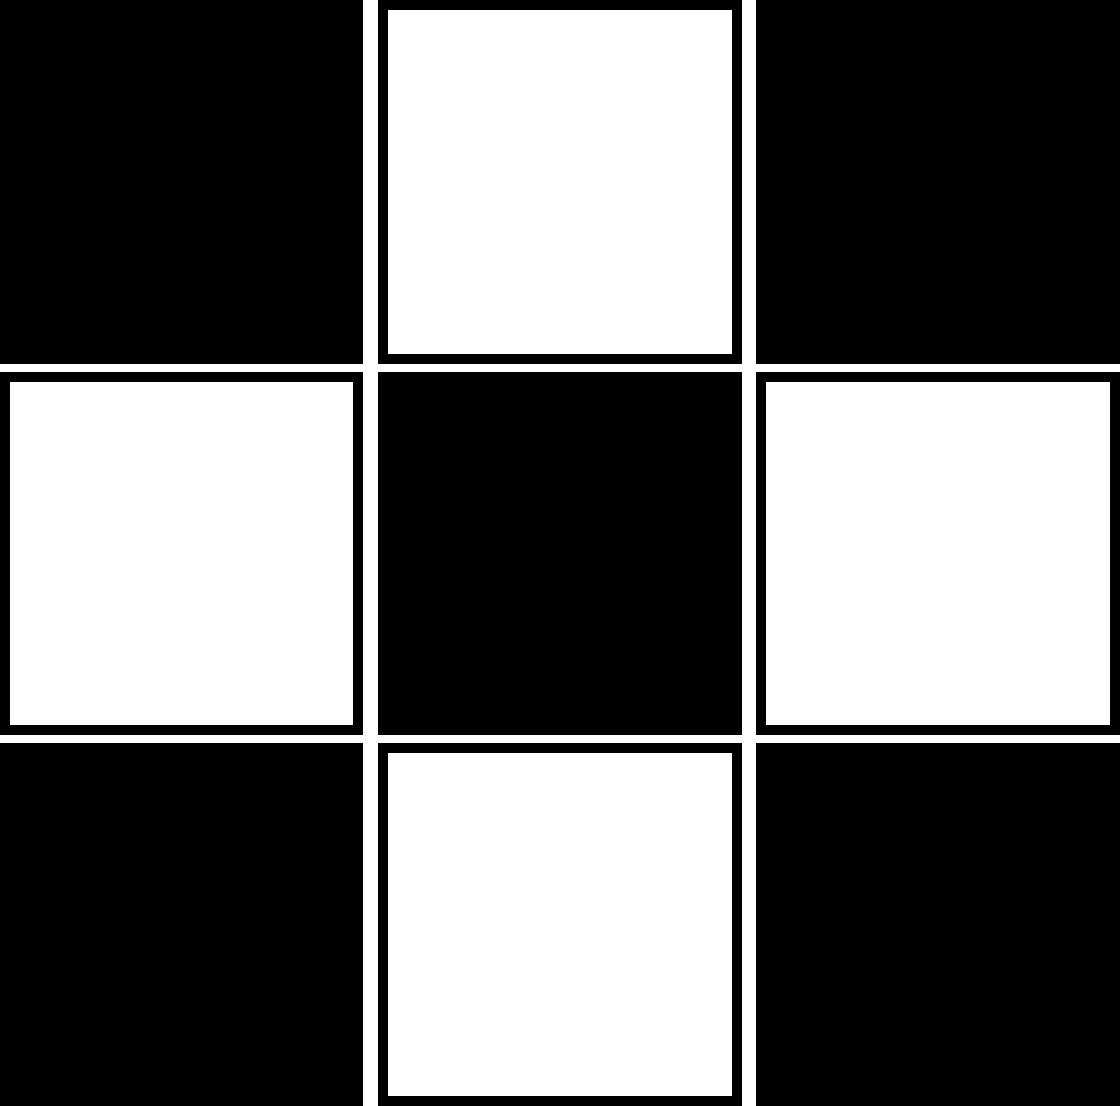
\includegraphics[width=0.1\textwidth]{../pictures/1.png} & 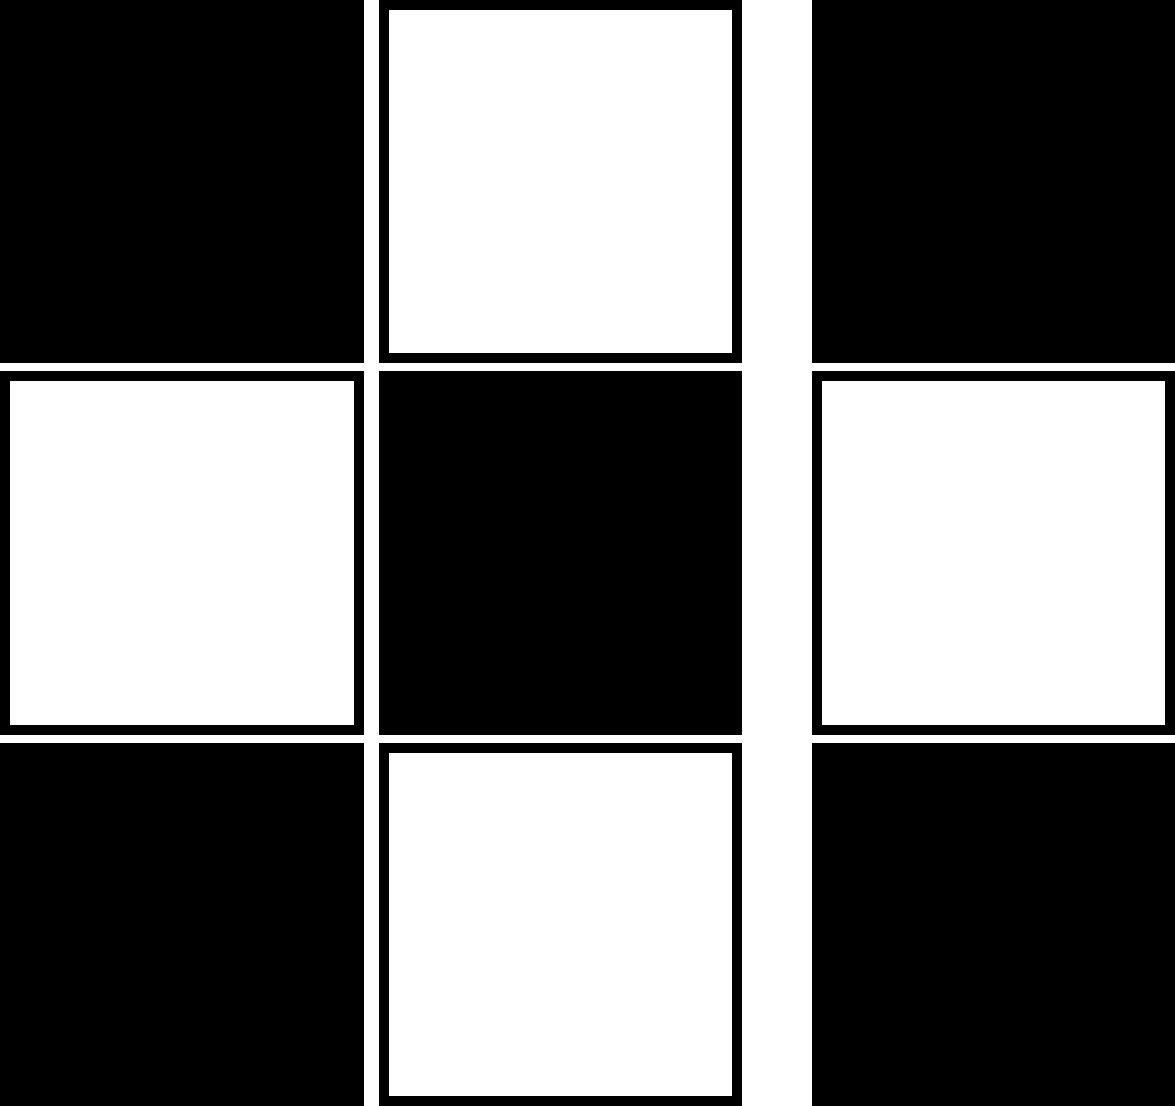
\includegraphics[width=0.1\textwidth]{../pictures/2.png} & 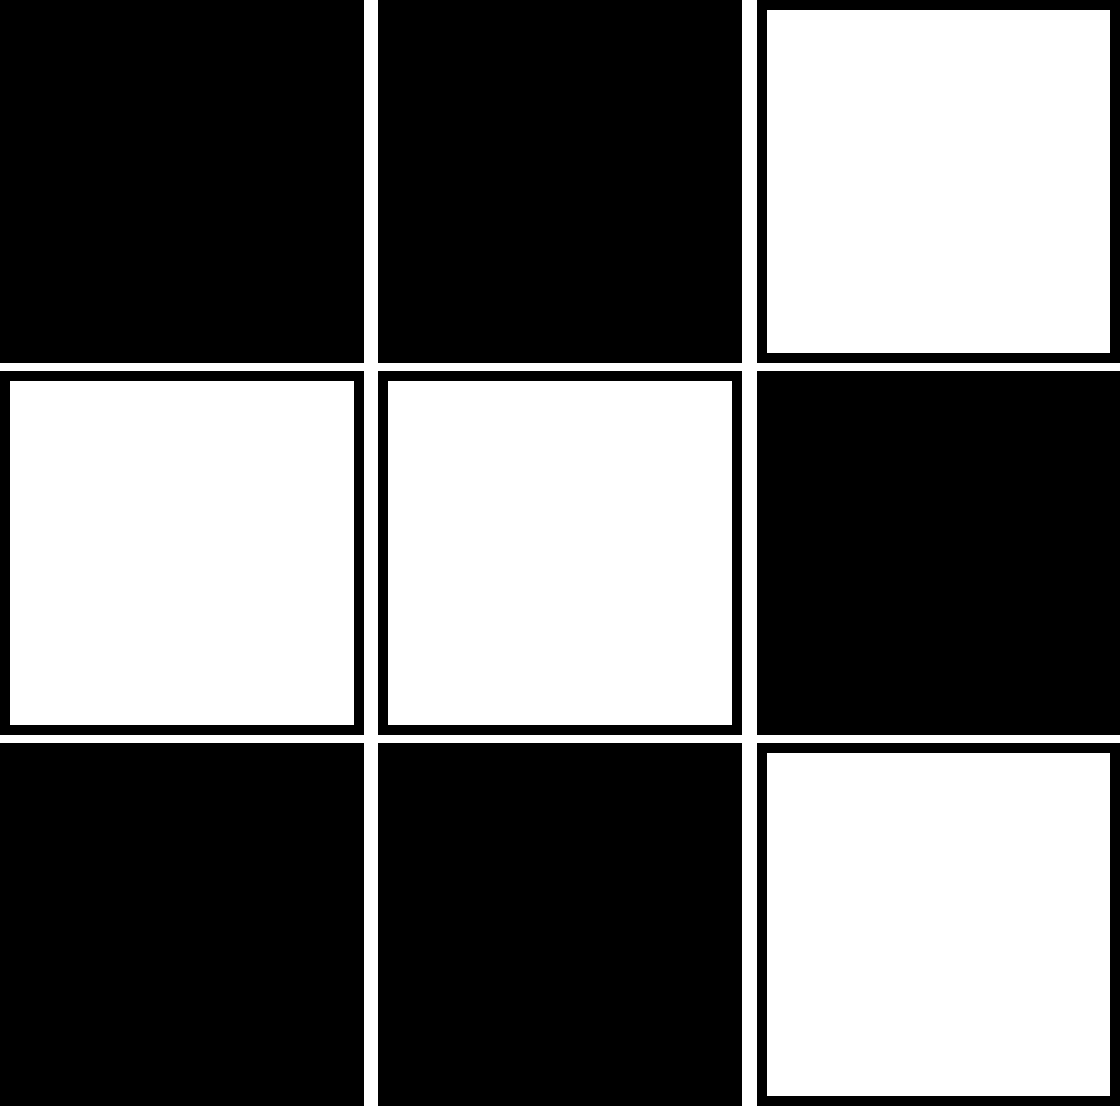
\includegraphics[width=0.1\textwidth]{../pictures/3.png} & 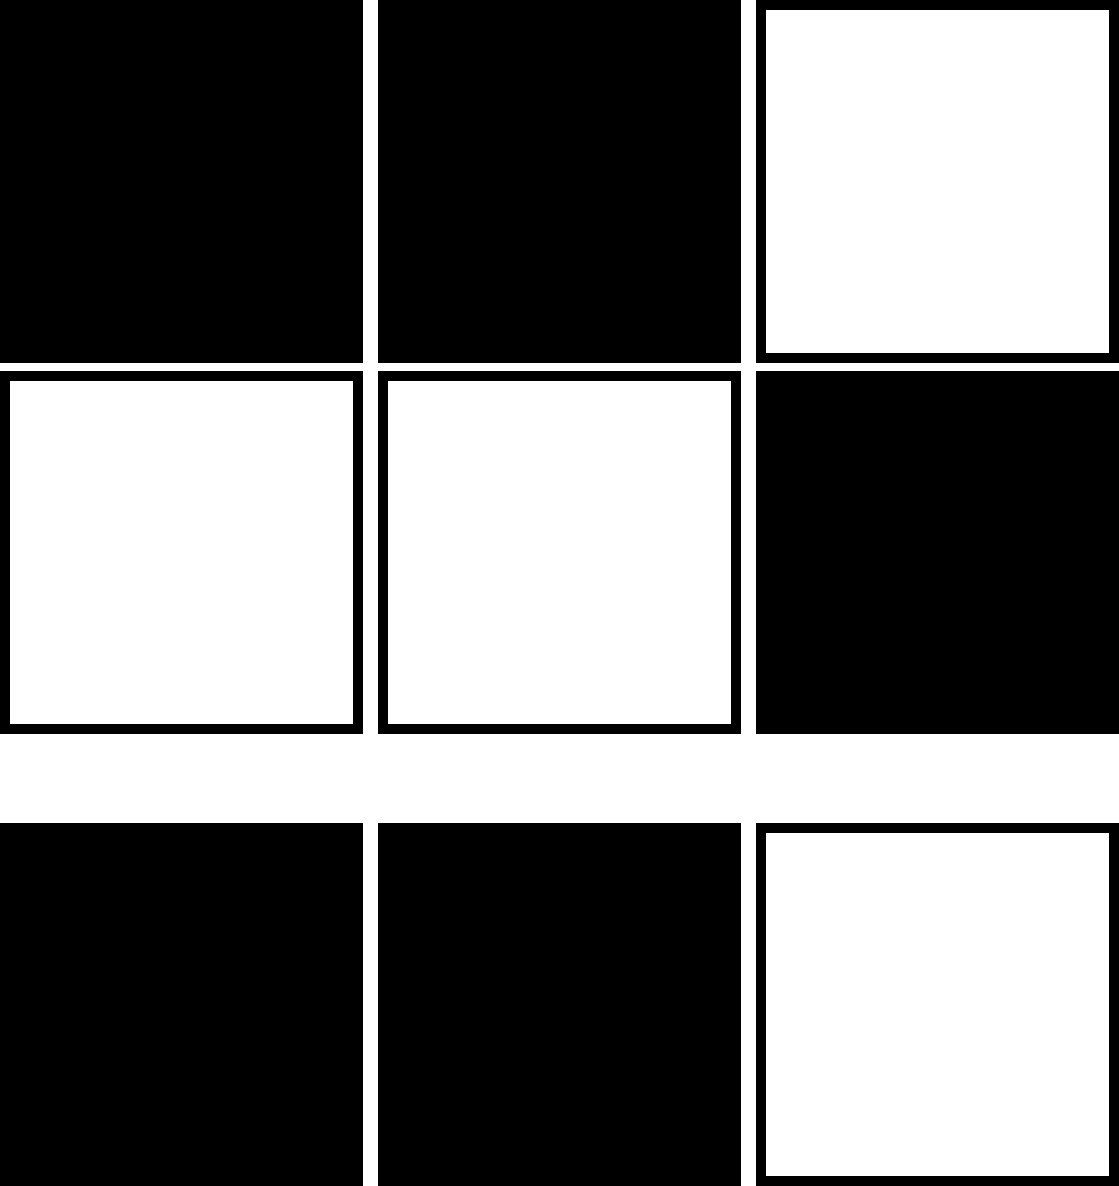
\includegraphics[width=0.1\textwidth]{../pictures/4.png} & 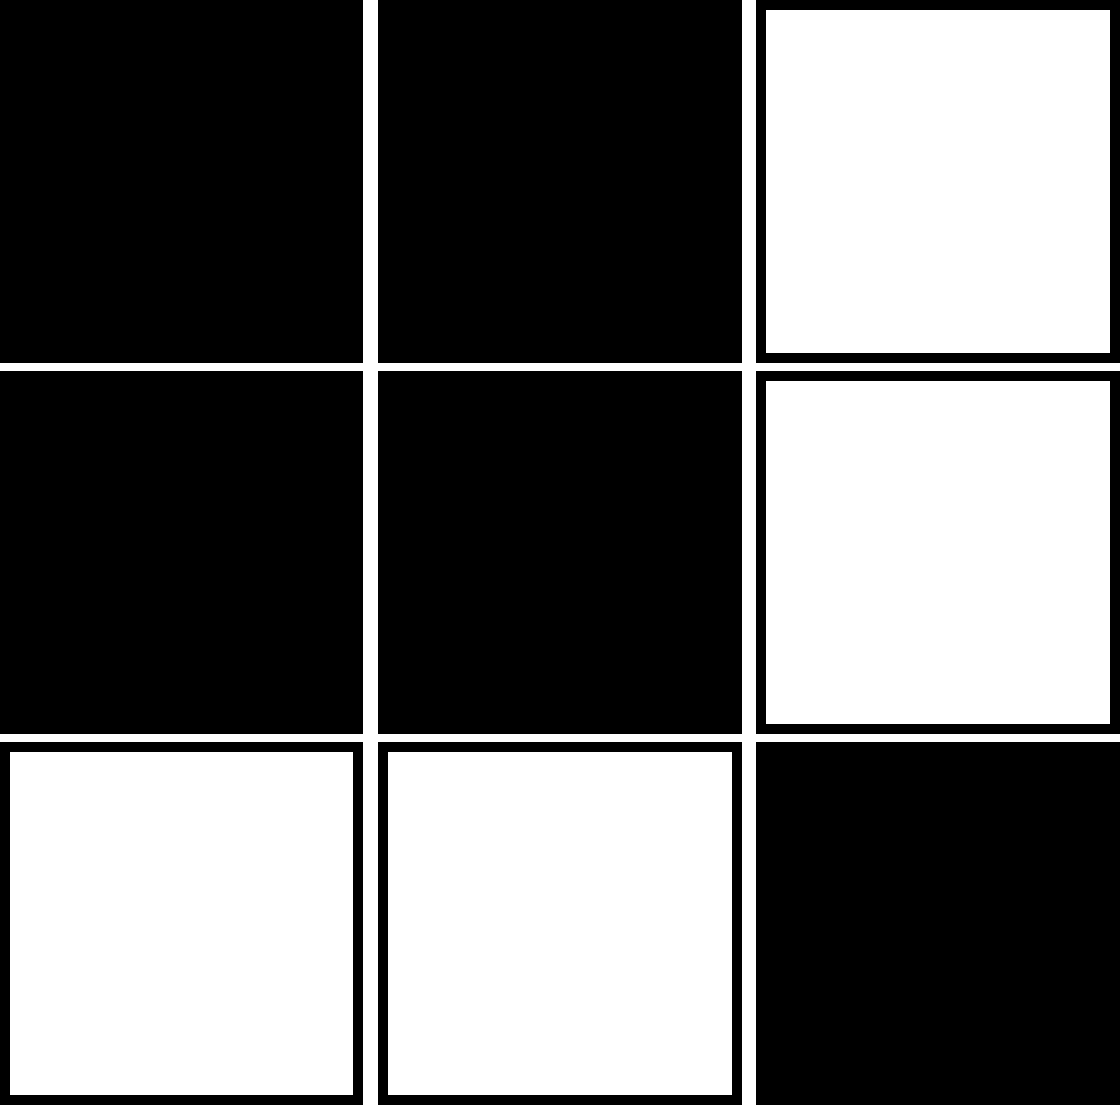
\includegraphics[width=0.1\textwidth]{../pictures/5.png}
\end{tabular}
\end{center}

첫 번째 입력에서, 위 그림처럼 맨 오른쪽 열을 떼어내 가장 왼쪽에 붙인 뒤, 맨 아래 행을 떼어내 가장 위쪽에 붙이면 크기 $4$의 정사각형을 만들 수 있다.

\end{problem}
